\begin{frame}
\section{Konzept}
\frametitle{Was ist Apache Kafka?}
\begin{columns}[T]
	\begin{column}[T]{0.49\textwidth}
		
	\end{column}
	\begin{column}[T]{0.49\textwidth}
		
\end{column}
\end{columns}

\centering
\begin{figure}[h]
	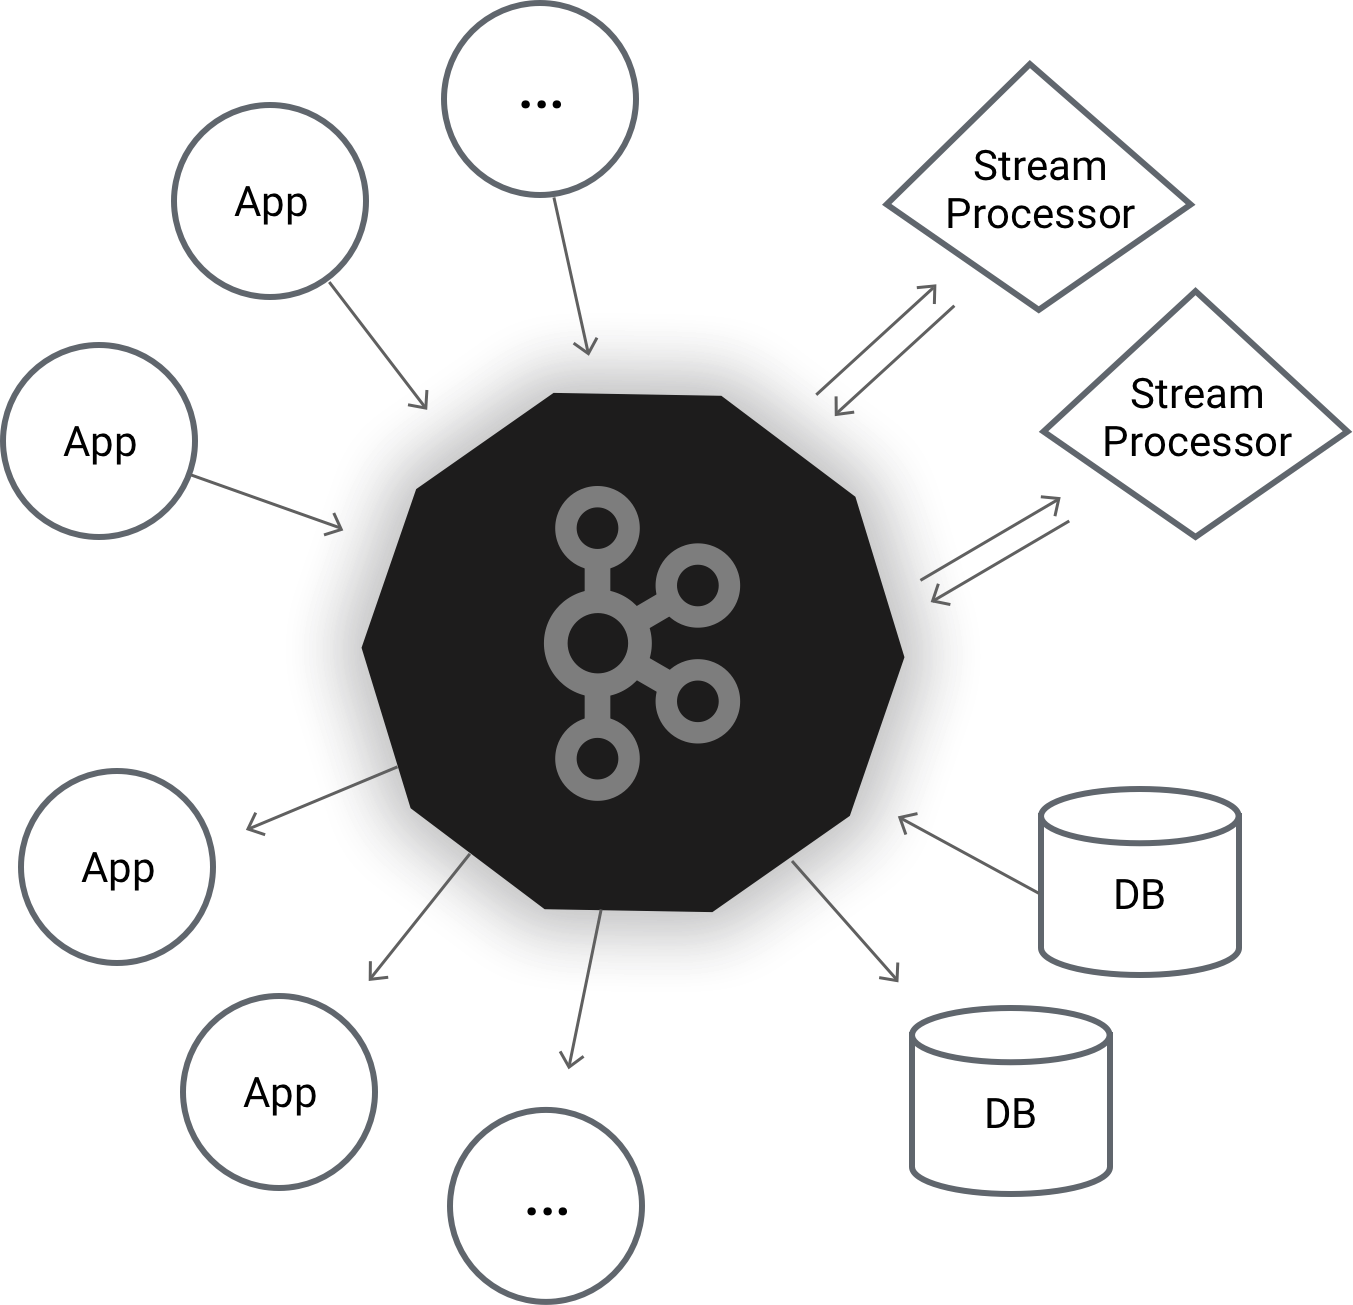
\includegraphics[scale=0.1]{figure/kafka_diagram.png}
\end{figure}

Apache Kafka ist eine verteilte skalierbare Streaming Plattform.
\end{frame}


\begin{frame}
\frametitle{Eigenschaften}
Kafka ...
\begin{itemize}
	\item ist ein Message Queuing System
	\item kann Nachrichten speichern
	\item kann Nachrichten verarbeiten
	\item kann all das in Echtzeit
\end{itemize}
\end{frame}

\begin{frame}
\frametitle{Unternehmen und Use Cases}
\begin{itemize}
	\item 
\includegraphics[scale=0.2]{figure/linkedin_logo.pdf} 
		- Operationsmetriken
	\item 
\includegraphics[scale=0.2]{figure/cisco_logo.pdf} 
		- OpenSOC (Security Operations Center)
	\item 
\includegraphics[scale=0.08]{figure/netflix_logo.pdf} 
		- Real-time monitoring and event-processing pipeline
	\item 
\includegraphics[scale=0.2]{figure/spotify_logo.pdf} 
		- Log Delivery System
	\item 
\includegraphics[scale=0.1]{figure/twitter_logo.pdf} 
		- Teil der Storm Stream Processing Infrastruktur
\end{itemize}
\end{frame}

\begin{frame}
\frametitle{Komponenten}
	\centering
	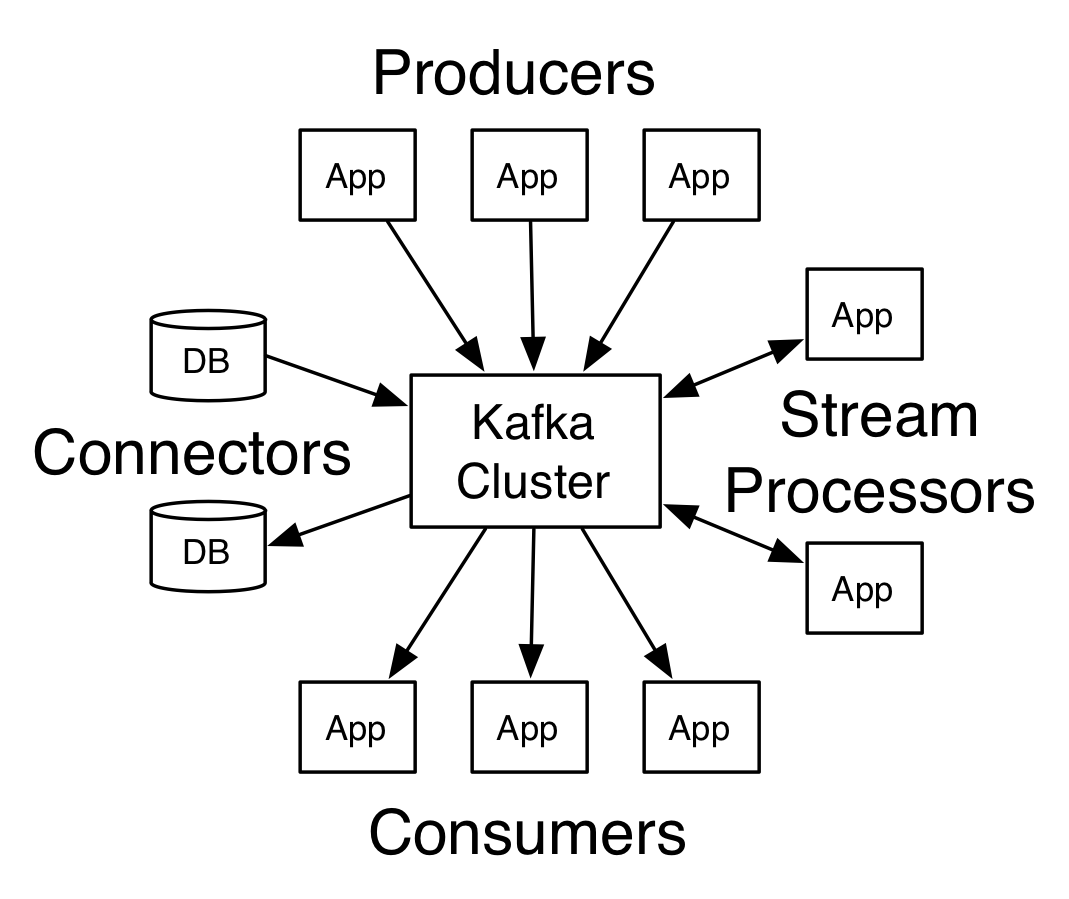
\includegraphics[scale=1.4]{figure/kafka-apis.png}
\end{frame}

\begin{frame}
\frametitle{Topics}
	\begin{center}
		B I L D
	\end{center}
\end{frame}

\begin{frame}
\frametitle{Kafka Topics}
\begin{itemize}
	\item Multi-Subscribe ($0$ bis $n$ Consumer)
	\item Kein Push-System
	\item Records in Topics werden persistent gehalten
	\item Topics benötigen eine Cleanup-Policy
		\begin{itemize}
			\item Retention-Time
			\item Retention-Size
			\item Log-Compaction
		\end{itemize}
	\item Topics besitzen Partitionen (partition log)
\end{itemize}
\end{frame}

\begin{frame}
\frametitle{Partitionen}

\end{frame}

\begin{frame}
\frametitle{Kafka Cluster}

\end{frame}